\documentclass[12pt]{standalone}
\usepackage{tikz}

\begin{document}

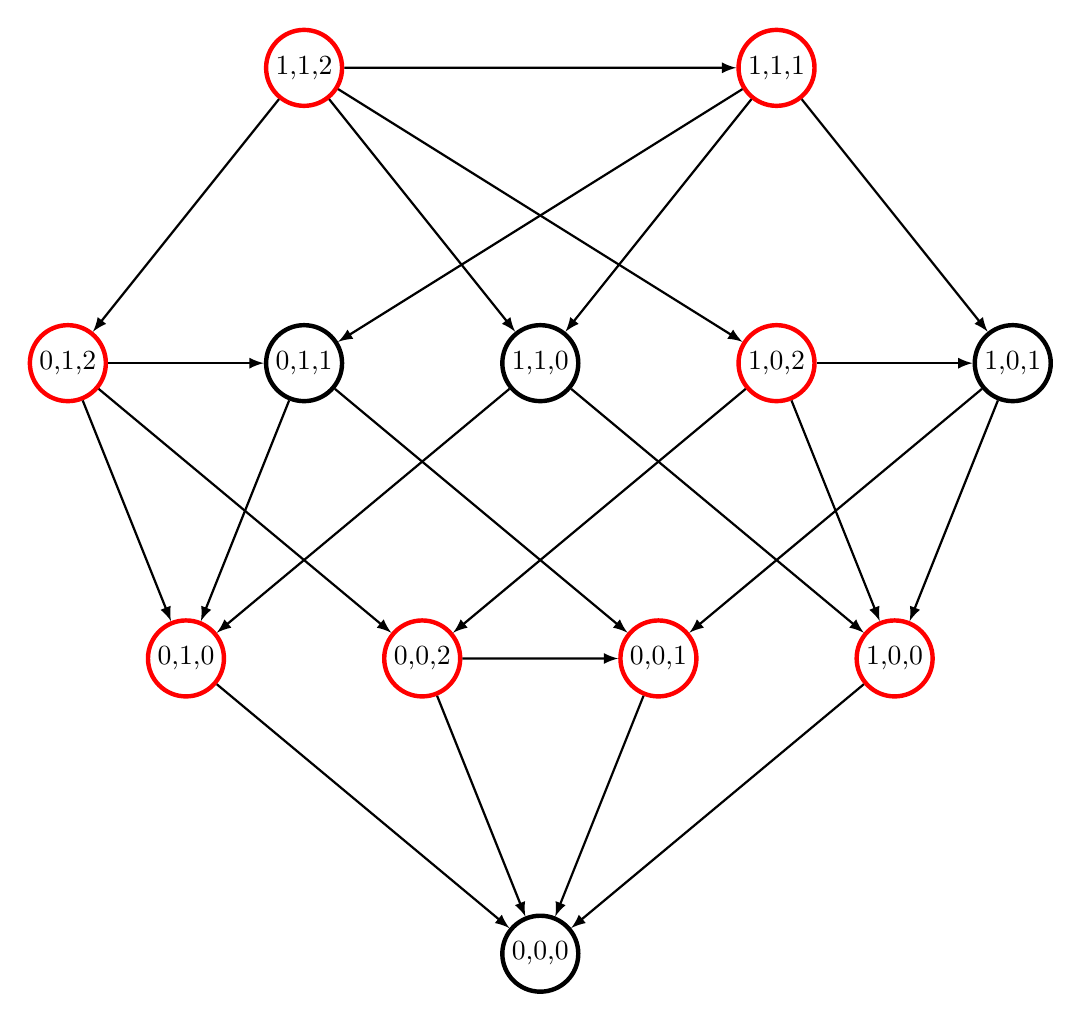
\begin{tikzpicture}[
    xscale=1.5, yscale=1.25,
    every node/.style={circle, ultra thick, draw, inner sep=2pt},
    every path/.style={thick, ->, >=latex},
]
% Nodes.
\node[draw=red] (112) at (-2, 3) {1,1,2};
\node[draw=red] (111) at ( 2, 3) {1,1,1};
\node[draw=red] (012) at (-4, 0) {0,1,2};
\node[draw=black] (011) at (-2, 0) {0,1,1};
\node[draw=black] (110) at ( 0, 0) {1,1,0};
\node[draw=red] (102) at ( 2, 0) {1,0,2};
\node[draw=black] (101) at ( 4, 0) {1,0,1};
\node[draw=red] (010) at (-3,-3) {0,1,0};
\node[draw=red] (002) at (-1,-3) {0,0,2};
\node[draw=red] (001) at ( 1,-3) {0,0,1};
\node[draw=red] (100) at ( 3,-3) {1,0,0};
\node[draw=black] (000) at ( 0,-6) {0,0,0};

% Edges.
\path (112) edge (012);
\path (012) edge (002);
\path (002) edge (001);
\path (001) edge (000);
\path (002) edge (000);
\path (012) edge (011);
\path (011) edge (001);
\path (011) edge (010);
\path (010) edge (000);
\path (012) edge (010);
\path (112) edge (102);
\path (102) edge (002);
\path (102) edge (101);
\path (101) edge (001);
\path (101) edge (100);
\path (100) edge (000);
\path (102) edge (100);
\path (112) edge (111);
\path (111) edge (011);
\path (111) edge (101);
\path (111) edge (110);
\path (110) edge (010);
\path (110) edge (100);
\path (112) edge (110);

\end{tikzpicture}

\end{document}